\documentclass[hyperref=colorlinks]{beamer}
\mode<presentation>
\usetheme{iclpt}
\setbeamertemplate{navigation symbols}{}
\setbeamertemplate{headline}{
\begin{beamercolorbox}[leftskip=.2cm,rightskip=.2cm,topskip=.2cm,ht=1.1cm,dp=0.1cm,wd=\textwidth]{institute in head/foot}
  
\includegraphics[height=1cm]{icl.pdf}
  \hfill
  
\includegraphics[height=1cm]{../Pics/CMS-Color.pdf}
\end{beamercolorbox}
}
\setbeamertemplate{footline}{
\begin{beamercolorbox}[ht=.55cm,dp=0.4cm,wd=\textwidth,leftskip=.3cm]{author in head/foot}%
  \begin{minipage}[c]{5cm}%
    \usebeamerfont{author in head/foot}
    \insertshortauthor 
    \insertshorttitle
    \end{minipage}\hfill%
  \insertframenumber{} / \pageref{lastframe}
  \hfill
  \begin{minipage}{6cm}
    \hfill
  \end{minipage}
\end{beamercolorbox}%
}

\usepackage{color}
\usepackage{tabularx,colortbl}
\usepackage{graphicx}
\usepackage{pdfpages}
\usepackage{feynmp}
\DeclareGraphicsRule{*}{mps}{*}{}

\title{\vspace{-0.2cm} VBF Higgs to Invisible - Update}
\subtitle{HIG-14-038, AN-14-243\vspace{-0.7cm}}
\author[P. Dunne]{\underline{P. Dunne}} % A.M. Magnan and A. Nikitenko Joao Pela with \\ R. Aggleton, J. Brooke: Bristol \\ C.Asawangtrakuldee, Q.Li: Peking \\ P. Srimanobhas: Chulalongkorn \\ S. Kumar, K. Mazumdar: Mumbai}
\titlegraphic{
  \vspace{-0.7cm}
  %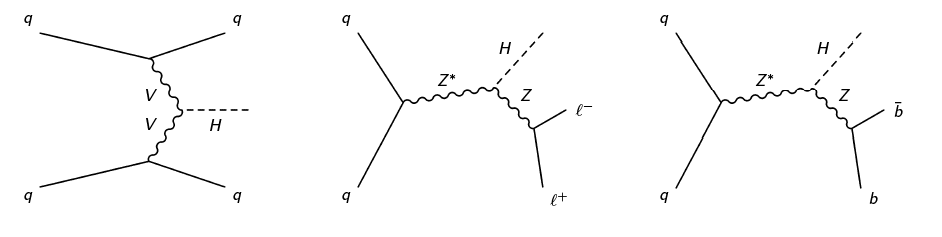
\includegraphics[width=\textwidth]{TalkPics/invcomb021213/feyndiags}
  %% \begin{fmfgraph*}(100,70)
  %%         \fmfleft{i1,i2}
  %%         \fmfright{o1,o2,o3}
  %%         \fmf{fermion}{i1,v1,o1}
  %%         \fmf{fermion}{i2,v2,o3}
  %%         \fmf{phantom,tension=4/5}{v1,v2}
  %%         \fmffreeze
  %%         \fmf{photon,label=$W,,Z$}{v1,v3}
  %%         \fmf{photon,label=$W,,Z$}{v2,v3}
  %%         \fmf{dashes}{v3,o2}
  %%         \fmflabel{$q$}{i1}
  %%         \fmflabel{$q$}{i2}
  %%         \fmflabel{$q$}{o1}
  %%         \fmflabel{$q$}{o3}
  %%         \fmflabel{$H$}{o2}
  %%       \end{fmfgraph*}
}
\date{}
\begin{document}
\begin{fmffile}{higgsexoupdatefeyndiags}

%TITLE PAGE
\section{Title}
\begin{frame}
  \titlepage
  
\end{frame}

\begin{frame}
  \frametitle{Overview}
  \begin{block}{}
    \scriptsize
    \begin{itemize}
    \item CADI line HIG-14-038 in place with AN and paper draft attached
    \item[-] Frozen for preapproval on Thursday
    \item Will show today work on studies asked for by Paolo:
    \item[-] Signal efficiency variation with PU
    \item[-] Muon veto efficiency in signal as a function of PU
    \item[-] First look at closure test
      
    \end{itemize}
  \end{block}
\end{frame}

%OUTLINE
\begin{frame}
  \frametitle{Signal efficiency as a function of PU}
  \begin{block}{}
    \centering
    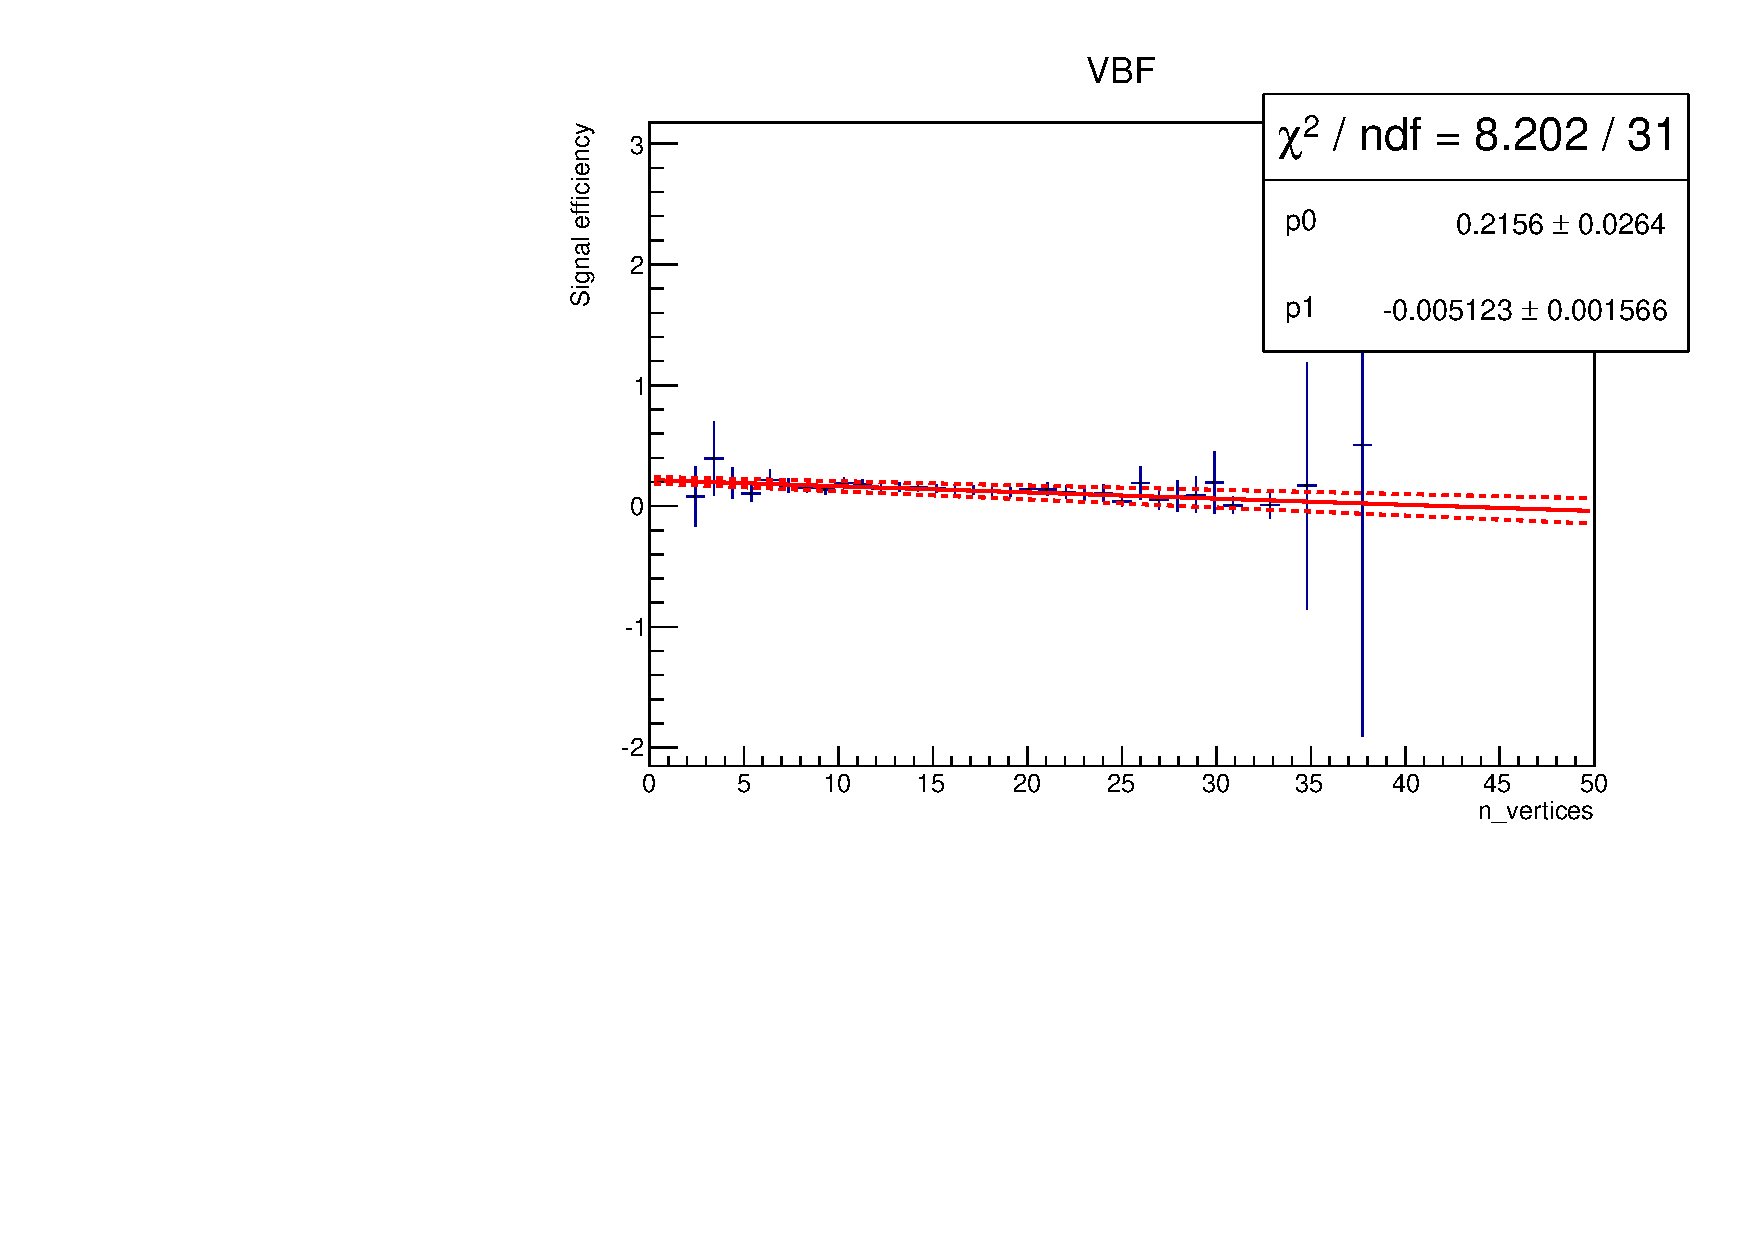
\includegraphics[width=.8\textwidth]{TalkPics/invupdate081214/vbfsigeff.pdf}
  \end{block}
\end{frame}

\begin{frame}
  \frametitle{Signal efficiency as a function of PU}
  \begin{block}{}
    \centering
    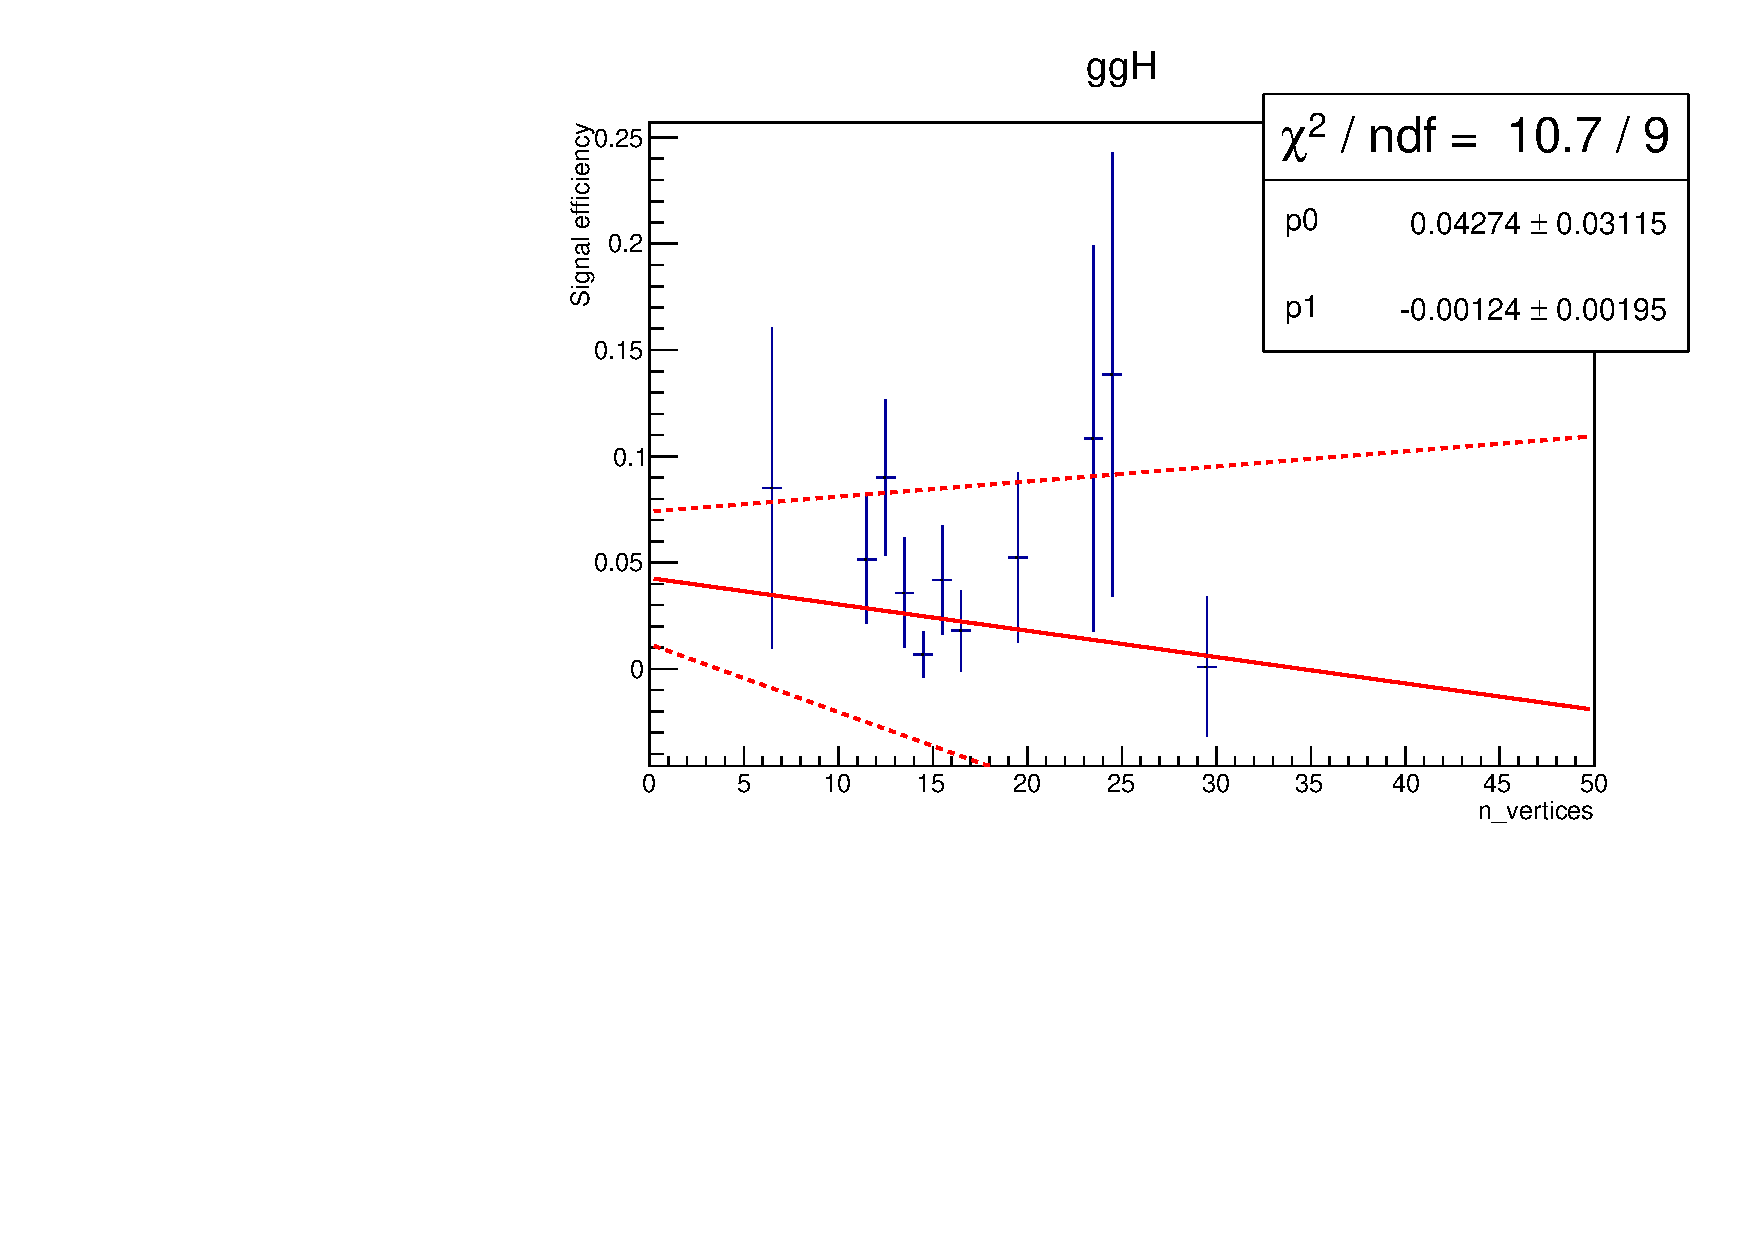
\includegraphics[width=.8\textwidth]{TalkPics/invupdate081214/gghsigeff.pdf}
  \end{block}
\end{frame}

\begin{frame}
  \frametitle{Veto muons in signal MC}
  \begin{block}{}
    \scriptsize
    \begin{itemize}
    \item Veto muons don't have a dz or dxy cut
    \item Concern that we would be vetoing muons from a different vertex
    \item Muon veto efficiency turns out to be very high:
    \item[-] $\sim$10 signal MC events with a veto muon out of $\sim$55000
    \item nvetomuons doesn't seem correlated with PU
    \end{itemize}
    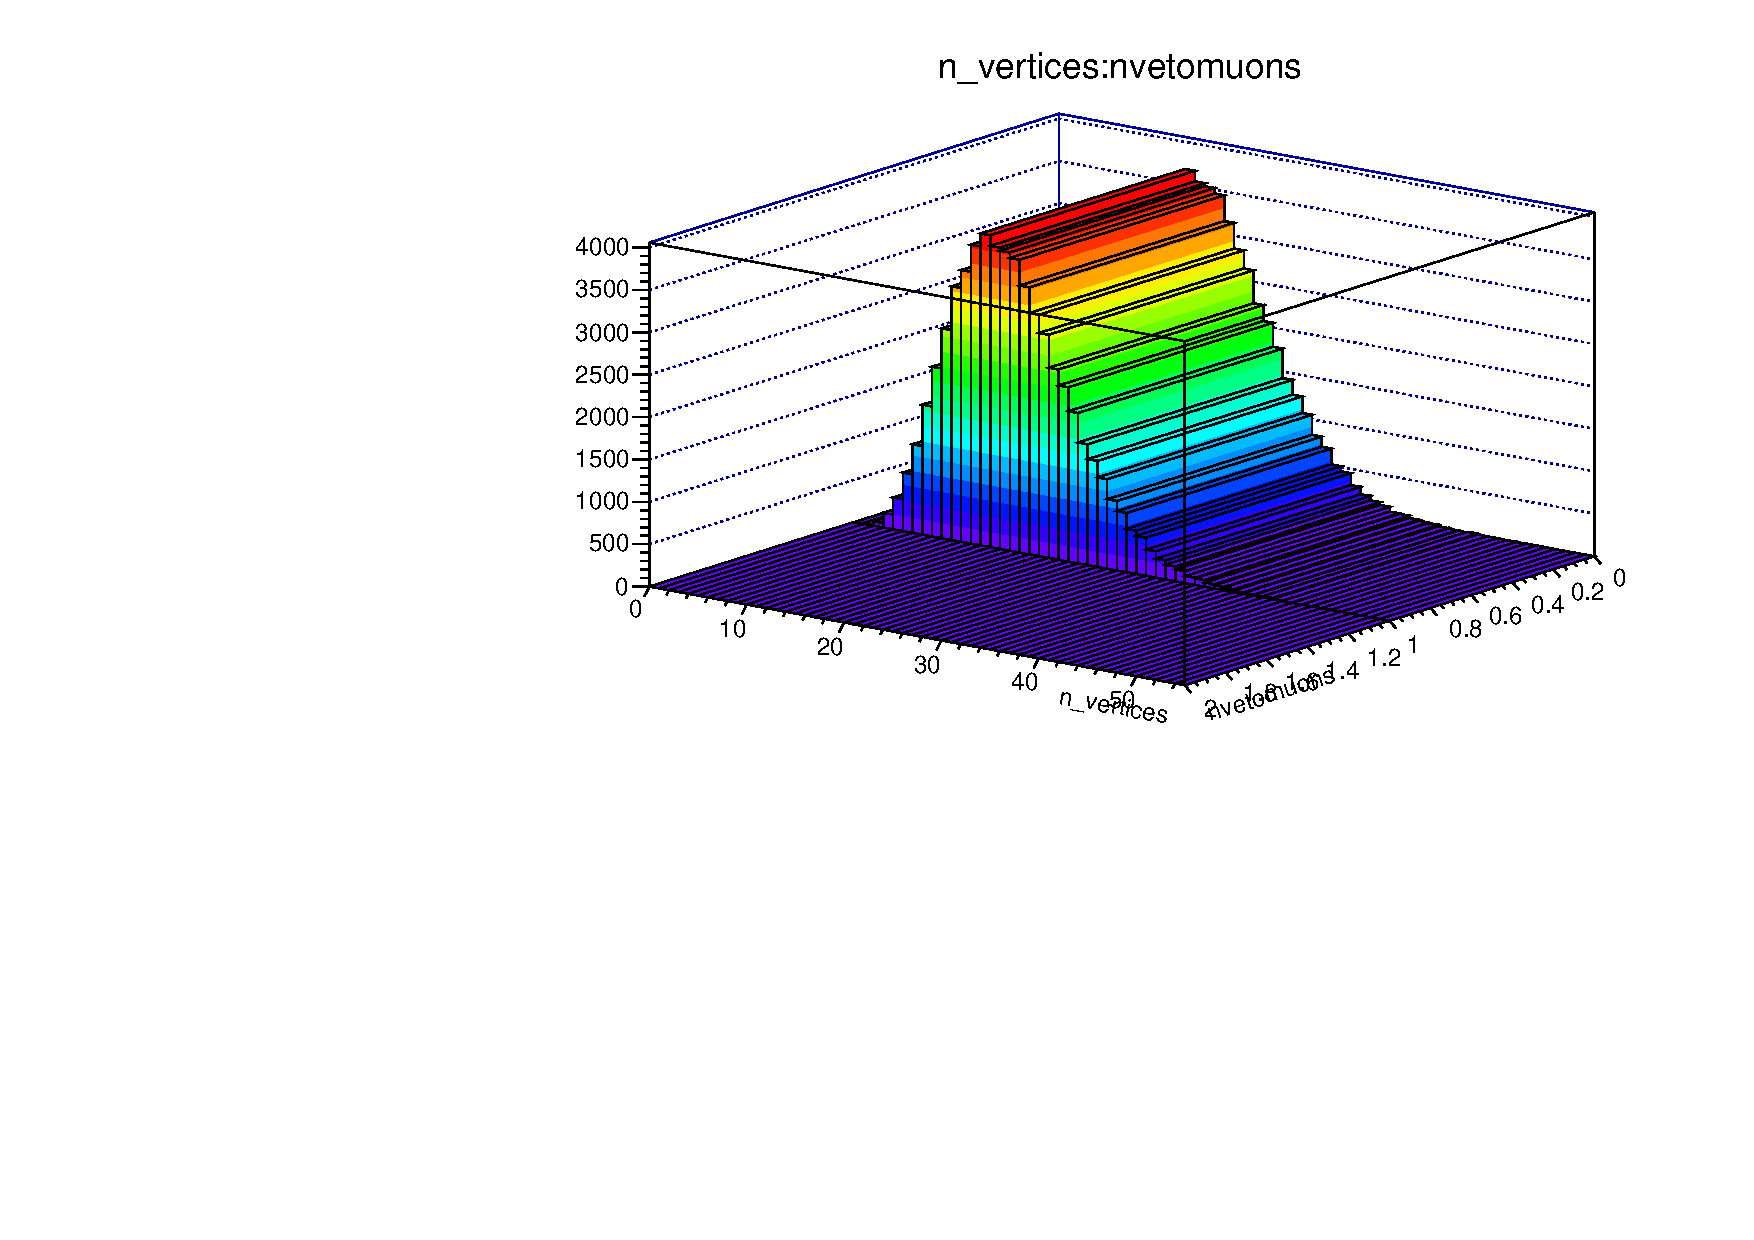
\includegraphics[width=.5\textwidth]{TalkPics/invupdate081214/vetomuvsPU.pdf}
    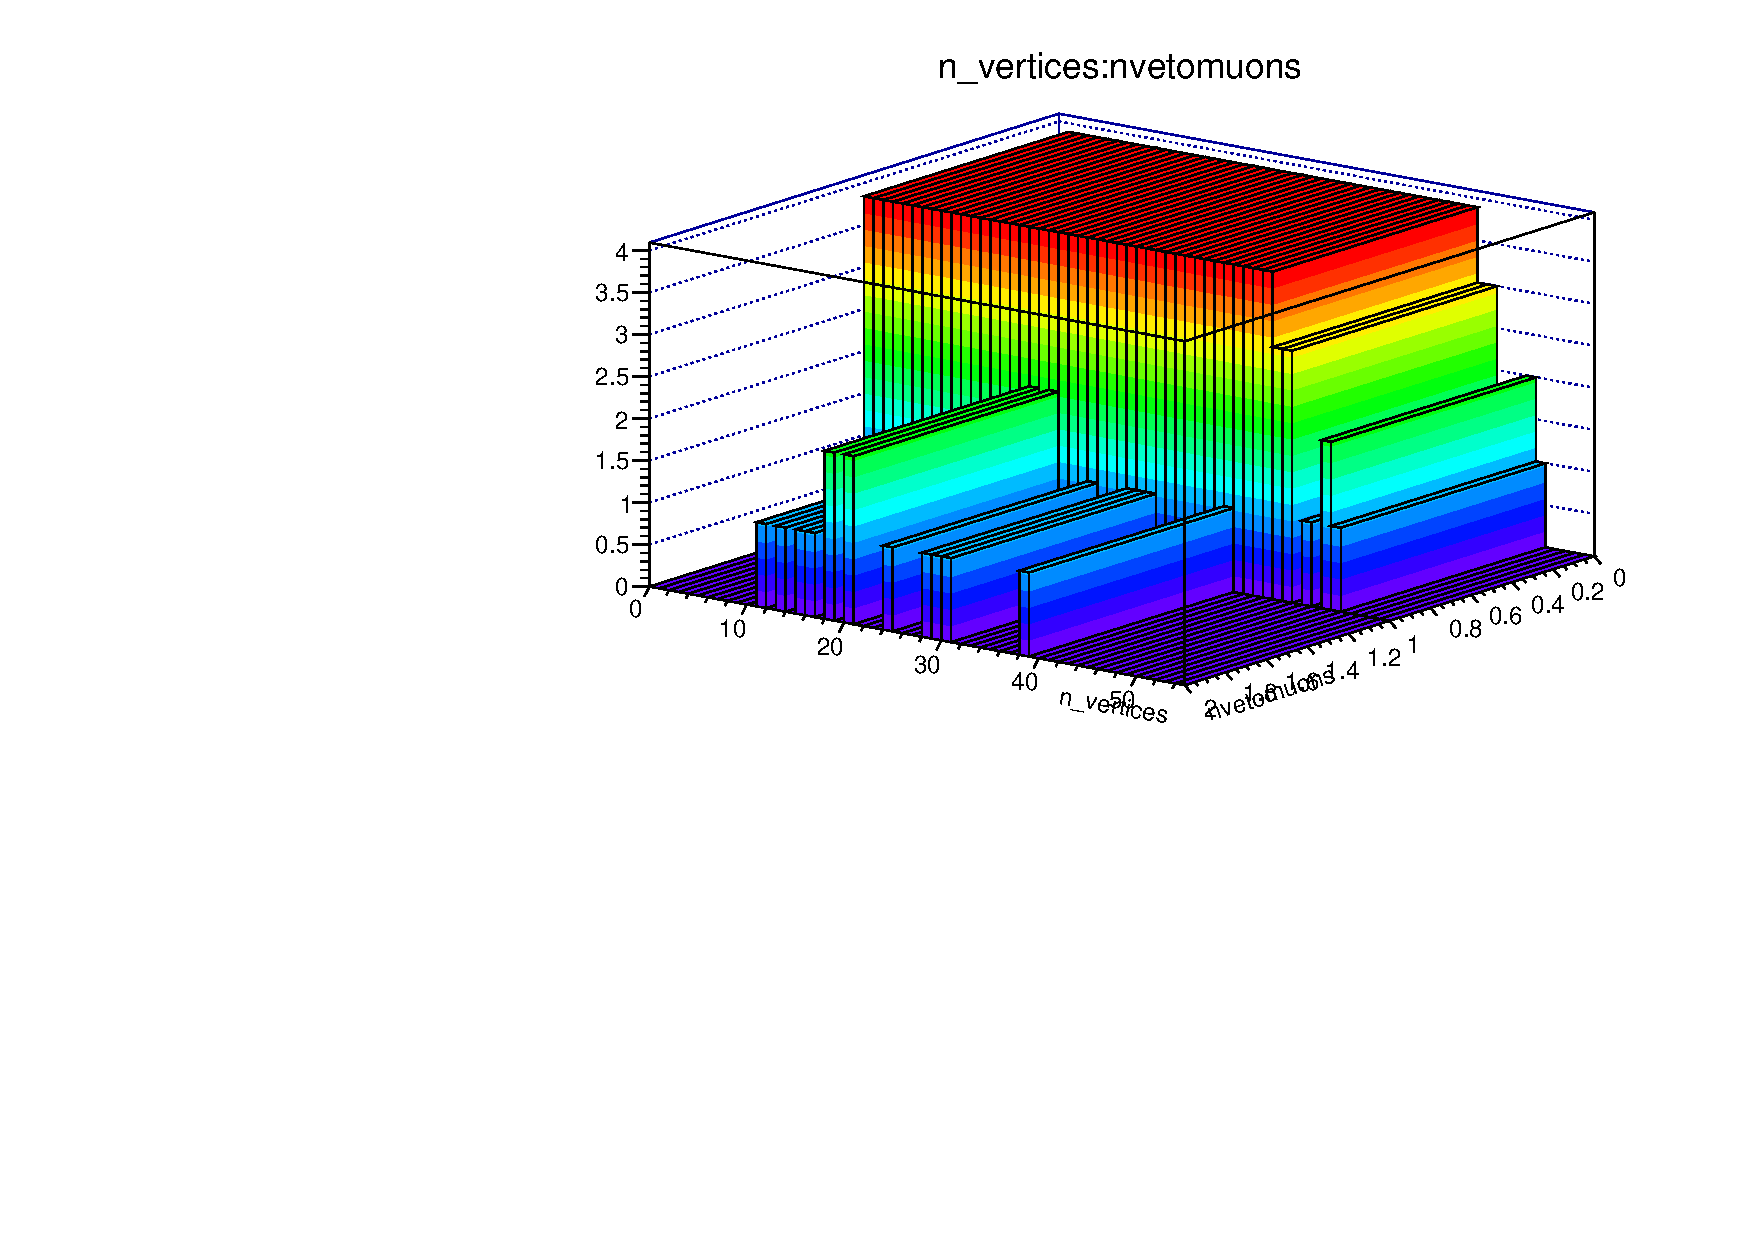
\includegraphics[width=.5\textwidth]{TalkPics/invupdate081214/vetomuvsPUzoom.pdf}
    \scriptsize
    \begin{itemize}
    \item Right plot is zoom of left
    \end{itemize}
  \end{block}
\end{frame}

\begin{frame}
  \frametitle{Closure tests}
  \begin{block}{}
    \scriptsize
    \begin{itemize}
    \item Use $W\rightarrow\mu\nu$ data driven weight for other backgrounds to check agreement
    \item For prompt analysis $W\rightarrow e\nu$ and $W\rightarrow\tau\nu$ agreed to 1$\sigma$
    \item[-] $Z\rightarrow\mu\mu$ was just outside error bands
    \item Instead of fitting a pol0 I have taken $\int$Data$/\int$MC
    \end{itemize}
  \end{block}
\end{frame}

\begin{frame}
  \frametitle{Closure tests}
  \begin{columns}
    \column{1.2\textwidth}
    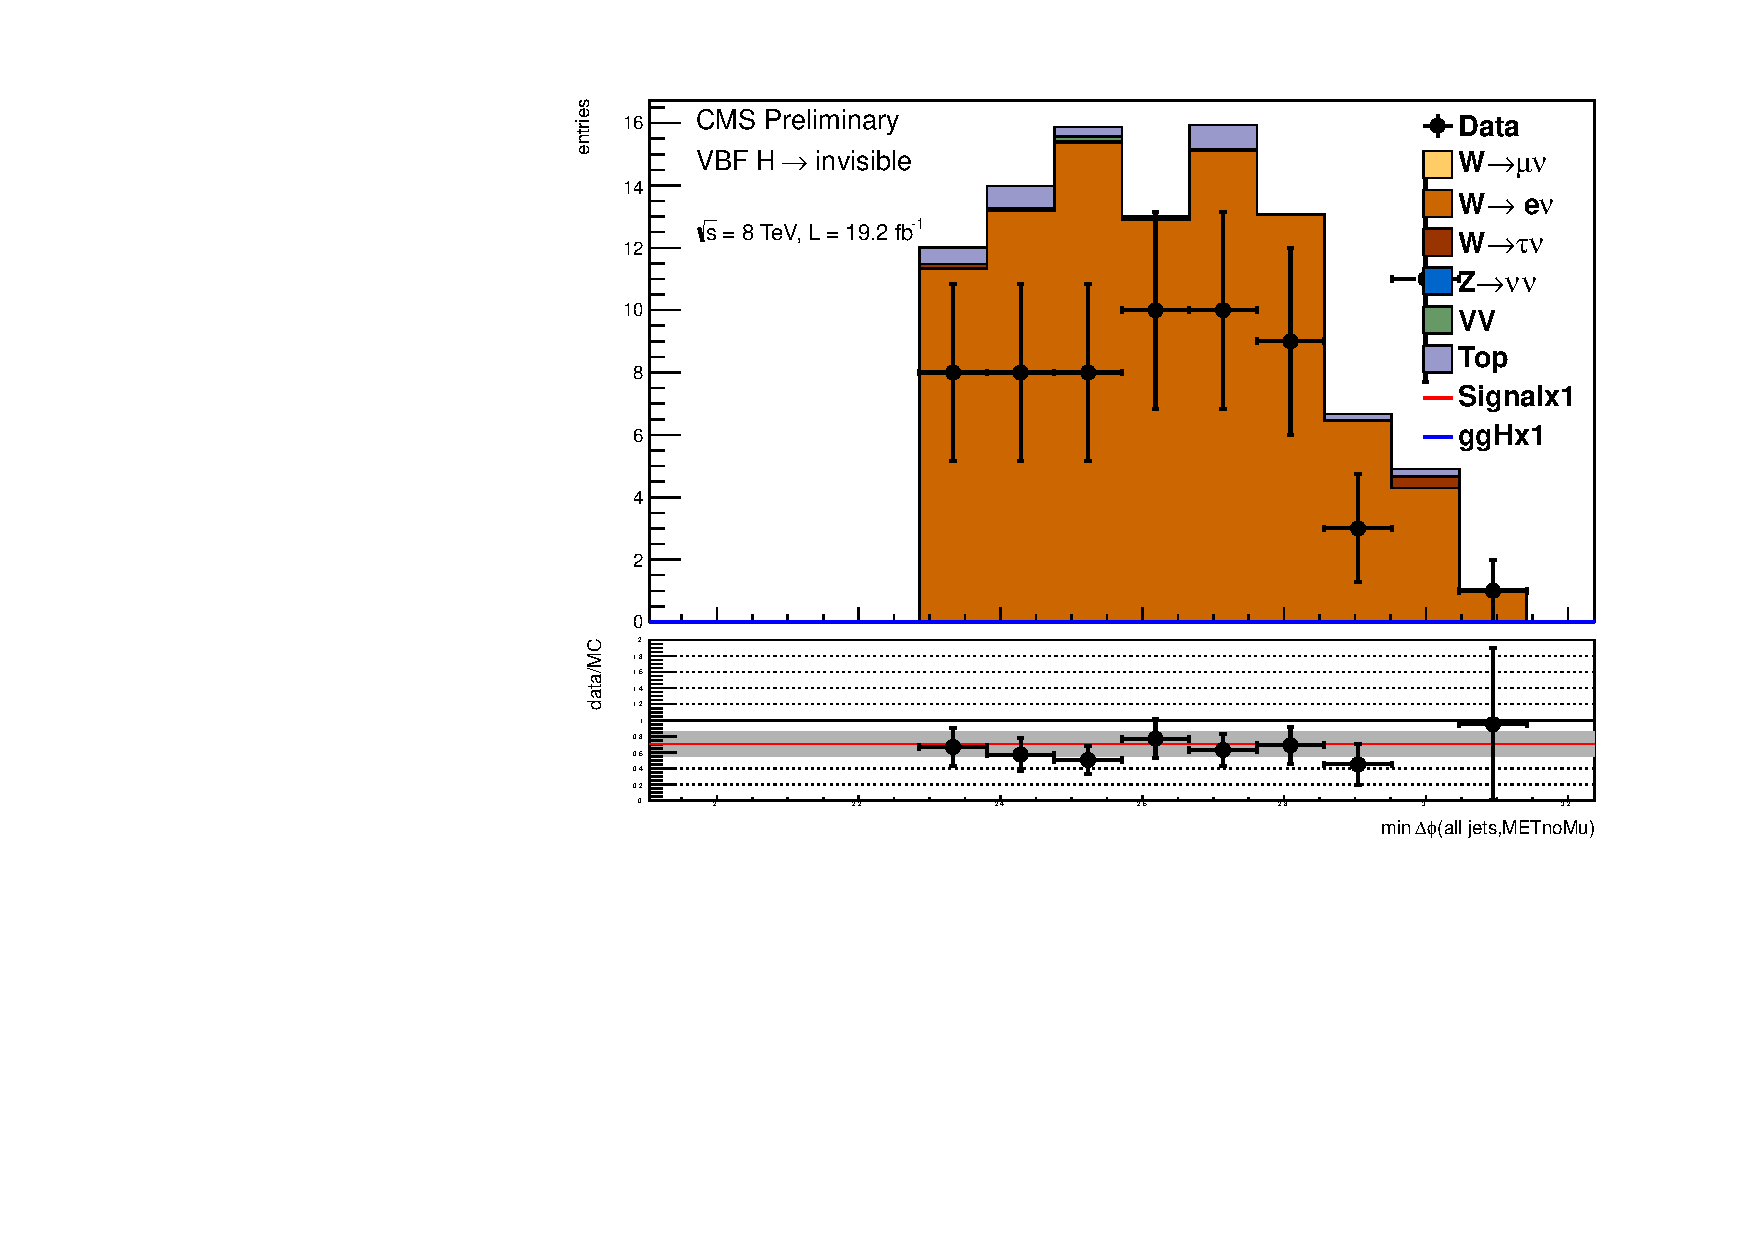
\includegraphics[width=.5\textwidth]{TalkPics/invupdate081214/enu_alljetsmetnomu_mindphi.pdf}
    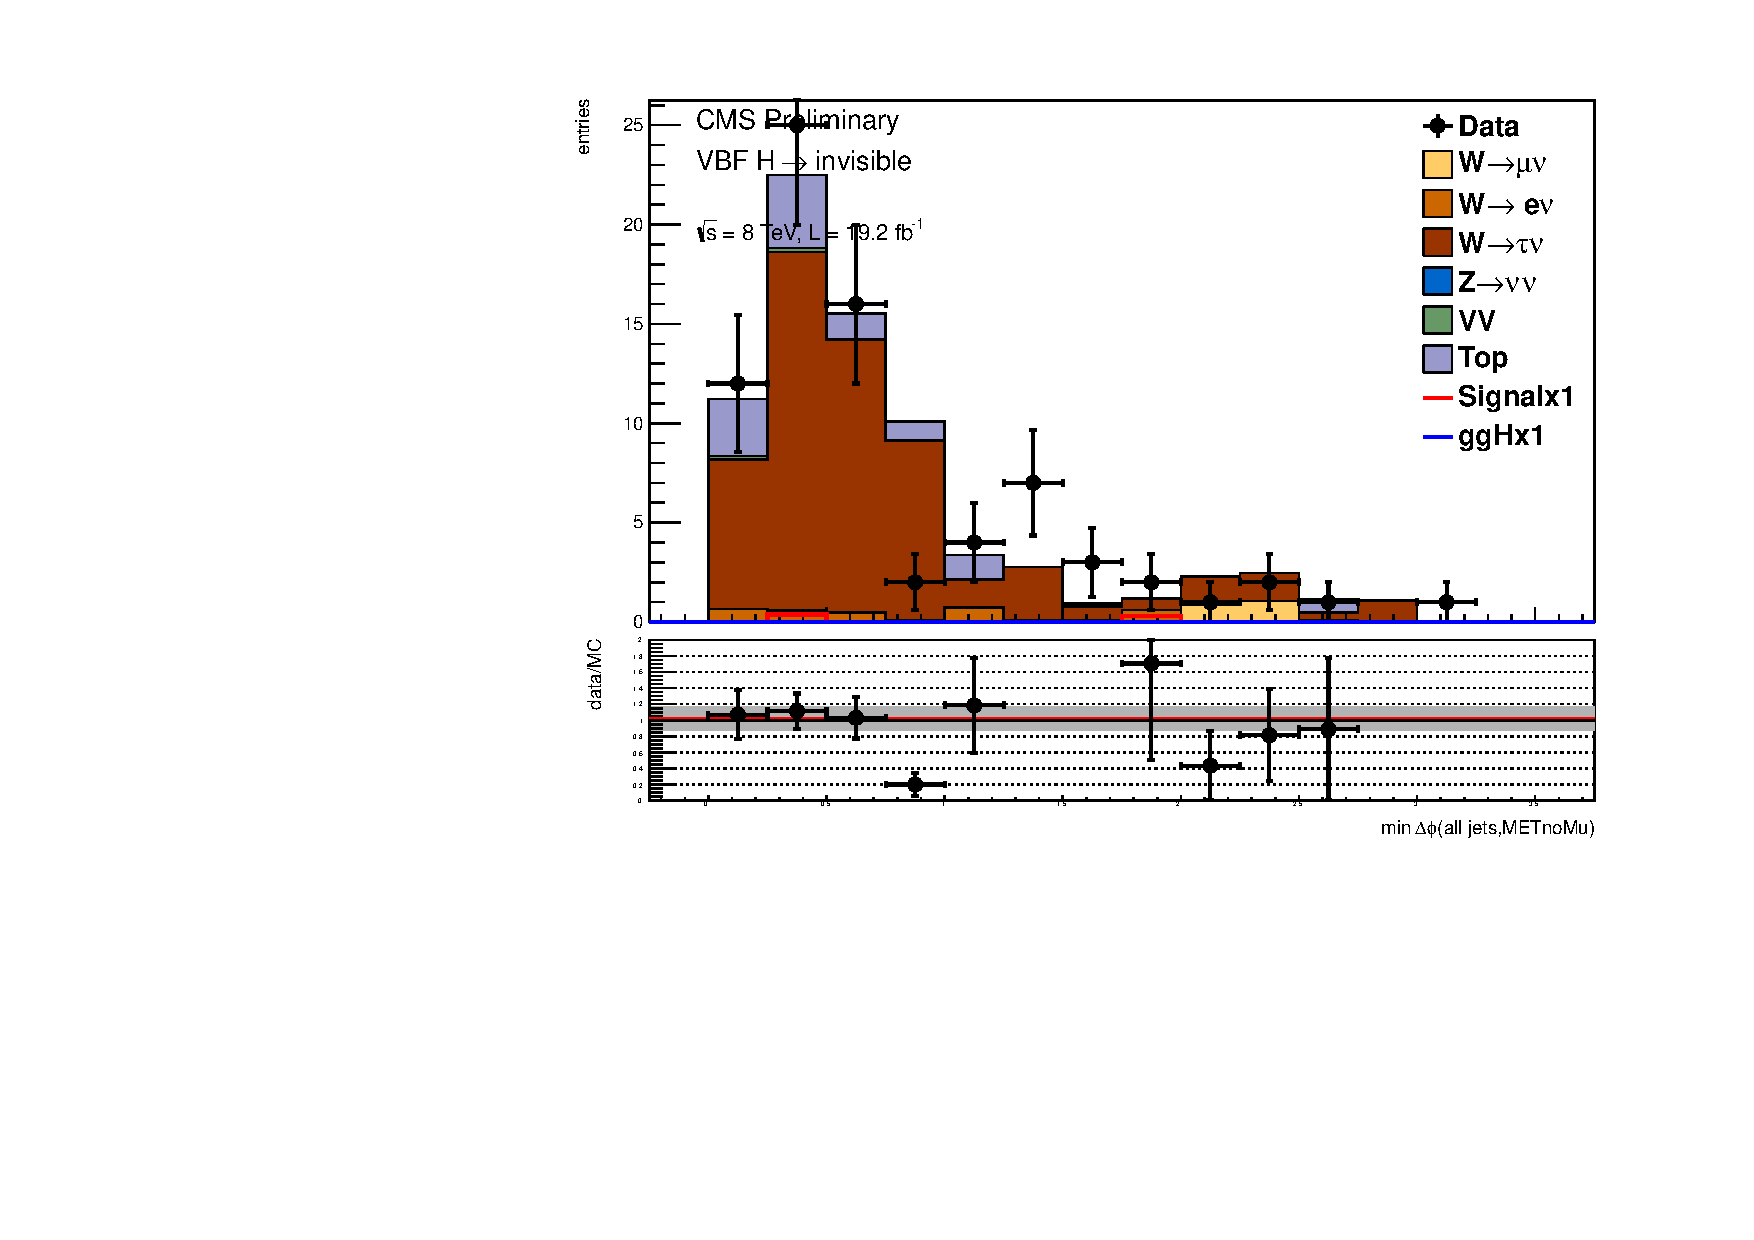
\includegraphics[width=.5\textwidth]{TalkPics/invupdate081214/taunu_alljetsmetnomu_mindphi.pdf}
    \end{columns}
  %!!PLOTS FOR ENU AND TAUNU
  %!!MENTION GOOD AGREEMENT ACROSS DPHIJJ, j2pt etc.
  %!!CHECKED electron and muon eta acceptance difference by adding a cut at 2.1 on both, no change
  %!!CHECKED QCD contamination with mt cut on enu region, no change
\end{frame}

\begin{frame}
  \frametitle{Closure tests}
  \begin{block}{}
    \scriptsize
    \begin{itemize}
    \item Errors shown are data and MC statistics only
    \item[-] Other errors are highly correlated
    \item Don't have $Z\rightarrow\mu\mu$ yet
    \item $W\rightarrow\tau\nu$ consistent to within errors
    \item $W\rightarrow e\nu$ shows $\sim 2\sigma$ difference
    \item[-] Flat across all variables
    \item Have tried adding an $m_{T}$ cut
    \item[-] no significant change
    \item Have tried adding an $\eta<2.1$ cut to make e and $\mu$ acceptance the same
    \item[-] No significant change
    \end{itemize}
  \end{block}
\end{frame}

\begin{frame}
  \frametitle{Conclusion}
  \label{lastframe}
  \begin{block}{}
    \scriptsize
    \begin{itemize}
    \item Muon veto shows no evidence of pileup dependancy
    \item Signal efficiency shows slight pileup dependancy
    \item[-] Not an issue as we model pileup distribution and uncertainty which gives a small systematic
    \item Closure tests underway
    \item[-] $W\rightarrow\tau\nu$ consistent
    \item[-] $W\rightarrow e\nu$ has 2$\sigma$ deviation
    \item Preapproval on Thursday
    \end{itemize}
    
  \end{block}

\end{frame}

\begin{frame}
  \frametitle{Backup}
\end{frame}

\end{fmffile}
\end{document}
